% This is "sig-alternate.tex" V2.1 April 20
% This file should be compiled with V2.5 of "sig-alternate.cls" May 2012
%
% This example file demonstrates the use of the 'sig-alternate.cls'
% V2.5 LaTeX2e document class file. It is for those submitting
% articles to ACM Conference Proceedings WHO DO NOT WISH TO
% STRICTLY ADHERE TO THE SIGS (PUBS-BOARD-ENDORSED) STYLE.
% The 'sig-alternate.cls' file will produce a similar-looking,
% albeit, 'tighter' paper resulting in, invariably, fewer pages.
%
% ----------------------------------------------------------------------------------------------------------------
% This .tex file (and associated .cls V2.5) produces:
%       1) The Permission Statement
%       2) The Conference (location) Info information
%       3) The Copyright Line with ACM data
%       4) NO page numbers
%
% as against the acm_proc_article-sp.cls file which
% DOES NOT produce 1) thru' 3) above.
%
% Using 'sig-alternate.cls' you have control, however, from within
% the source .tex file, over both the CopyrightYear
% (defaulted to 200X) and the ACM Copyright Data
% (defaulted to X-XXXXX-XX-X/XX/XX).
% e.g.
% \CopyrightYear{2007} will cause 2007 to appear in the copyright line.
% \crdata{0-12345-67-8/90/12} will cause 0-12345-67-8/90/12 to appear in the copyright line.
%
% ---------------------------------------------------------------------------------------------------------------
% This .tex source is an example which *does* use
% the .bib file (from which the .bbl file % is produced).
% REMEMBER HOWEVER: After having produced the .bbl file,
% and prior to final submission, you *NEED* to 'insert'
% your .bbl file into your source .tex file so as to provide
% ONE 'self-contained' source file.
%
% ================= IF YOU HAVE QUESTIONS =======================
% Questions regarding the SIGS styles, SIGS policies and
% procedures, Conferences etc. should be sent to
% Adrienne Griscti (griscti@acm.org)
%
% Technical questions _only_ to
% Gerald Murray (murray@hq.acm.org)
% ===============================================================
%
% For tracking purposes - this is V2.0 - May 2012

\documentclass{sig-alternate-05-2015}

\usepackage[usenames,dvipsnames]{xcolor}
\usepackage{listings}
\usepackage{relsize}
\usepackage{xspace}

\pdfcompresslevel0

\protected\def\CPP{C\nolinebreak[4]\hspace{-.04em}\raisebox{.21ex}{\relsize{-1.5}{\textbf{++}}}\xspace}

\begin{document}

% Copyright
\setcopyright{acmcopyright}
%\setcopyright{acmlicensed}
%\setcopyright{rightsretained}
%\setcopyright{usgov}
%\setcopyright{usgovmixed}
%\setcopyright{cagov}
%\setcopyright{cagovmixed}


% DOI
%\doi{10.475/123_4}

% ISBN
%\isbn{123-4567-24-567/08/06}

%Conference
\conferenceinfo{SAICSIT '15}{September 28--30, 2015, Stellenbosch, ZAR}

%\acmPrice{\$15.00}

%
% --- Author Metadata here ---
%\conferenceinfo{WOODSTOCK}{'97 El Paso, Texas USA}
%\CopyrightYear{2007} % Allows default copyright year (20XX) to be over-ridden - IF NEED BE.
%\crdata{0-12345-67-8/90/01}  % Allows default copyright data (0-89791-88-6/97/05) to be over-ridden - IF NEED BE.
% --- End of Author Metadata ---

\title{CAPP : C++ Aspect-Oriented Parallel Programming with AspectC++ and OpenCL}
%\subtitle{[Extended Abstract]
%\titlenote{A full version of this paper is available as
%\textit{Author's Guide to Preparing ACM SIG Proceedings Using
%\LaTeX$2_\epsilon$\ and BibTeX} at
%\texttt{www.acm.org/eaddress.htm}}}
%
% You need the command \numberofauthors to handle the 'placement
% and alignment' of the authors beneath the title.
%
% For aesthetic reasons, we recommend 'three authors at a time'
% i.e. three 'name/affiliation blocks' be placed beneath the title.
%
% NOTE: You are NOT restricted in how many 'rows' of
% "name/affiliations" may appear. We just ask that you restrict
% the number of 'columns' to three.
%
% Because of the available 'opening page real-estate'
% we ask you to refrain from putting more than six authors
% (two rows with three columns) beneath the article title.
% More than six makes the first-page appear very cluttered indeed.
%
% Use the \alignauthor commands to handle the names
% and affiliations for an 'aesthetic maximum' of six authors.
% Add names, affiliations, addresses for
% the seventh etc. author(s) as the argument for the
% \additionalauthors command.
% These 'additional authors' will be output/set for you
% without further effort on your part as the last section in
% the body of your article BEFORE References or any Appendices.

\numberofauthors{2} %  in this sample file, there are a *total*
% of EIGHT authors. SIX appear on the 'first-page' (for formatting
% reasons) and the remaining two appear in the \additionalauthors section.
%
\author{
% You can go ahead and credit any number of authors here,
% e.g. one 'row of three' or two rows (consisting of one row of three
% and a second row of one, two or three).
%
% The command \alignauthor (no curly braces needed) should
% precede each author name, affiliation/snail-mail address and
% e-mail address. Additionally, tag each line of
% affiliation/address with \affaddr, and tag the
% e-mail address with \email.
%
% 1st. author
\alignauthor
Author 1
\alignauthor 
Author 2
}
% There's nothing stopping you putting the seventh, eighth, etc.
% author on the opening page (as the 'third row') but we ask,
% for aesthetic reasons that you place these 'additional authors'
% in the \additional authors block, viz.
%\additionalauthors{Additional authors: John Smith (The Th{\o}rv{\"a}ld Group,
%email: {\texttt{jsmith@affiliation.org}}) and Julius P.~Kumquat
%(The Kumquat Consortium, email: {\texttt{jpkumquat@consortium.net}}).}
\date{\today}
% Just remember to make sure that the TOTAL number of authors
% is the number that will appear on the first page PLUS the
% number that will appear in the \additionalauthors section.

\maketitle
\begin{abstract}
	Parallel programming can provide higher computational performance over
	a sequential implementation by making use of the many cores available in
	parallel systems. However, the parallel-capable devices introduce complexity
	into the programming model. Current parallel programming API's such 
	as OpenCL and CUDA provide interfaces to the parallel devices, but are
	complex and result in code which includes cross-cutting components, 
	such as setting up the parallel programming context, compiling the parallel 
	kernel, and transferring data between the host and device memory spaces 
	when the kernel is executed. A \CPP Aspect-Oriented Parallel Programming
	(CAPP) model is developed, using Aspect\CPP and OpenCL, which defines aspects to 
	remove the cross-cutting components from  the \CPP code. The aspects set
	up the OpenCL context, compile the OpenCL kernel, and manage the data transfer 
	between the memory spaces each time a kernel is executed. The aspects are woven 
	into the \CPP code before compilation, rather than at run time, which improves 
	performance. An interface is provided for executing OpenCL kernels from the 
	\CPP code, essentially providing parallel programming in \CPP. The model was 
	applied to the SAXPY and Black-Scholes option pricing problems. Computational 
	performance was, on average, 1.4-7\% slower than the OpenCL implementation
	and up to 9 times faster than the sequential \CPP implementation for the
	Black-Scholes problem. The amount of code was greatly reduced from the OpenCL 
	implementation, and the resulting CAPP model \CPP code was simple and modular, 
	resembling the sequential \CPP implementation code.
\end{abstract}


%
% The code below should be generated by the tool at
% http://dl.acm.org/ccs.cfm
% Please copy and paste the code instead of the example below. 
%

\begin{CCSXML}
	<ccs2012>
	<concept>
	<concept_id>10010147.10010169.10010175</concept_id>
	<concept_desc>Computing methodologies~Parallel programming
	languages</concept_desc>
	<concept_significance>500</concept_significance>
	</concept>
	<concept>
	<concept_id>10010520.10010521.10010528</concept_id>
	<concept_desc>Computer systems organization~Parallel
	architectures</concept_desc>
	<concept_significance>300</concept_significance>
	</concept>
	<concept>
	<concept_id>10011007.10011006.10011050</concept_id>
	<concept_desc>Software and its engineering~Context specific
	languages</concept_desc>
	<concept_significance>300</concept_significance>
	</concept>
	</ccs2012>
\end{CCSXML}

\ccsdesc[500]{Computing methodologies~Parallel programming languages}
\ccsdesc[300]{Computer systems organization~Parallel architectures}
\ccsdesc[300]{Software and its engineering~Context specific languages}
%
% End generated code
%

%
%  Use this command to print the description
%
\printccsdesc

% We no longer use \terms command
%\terms{Theory}

\keywords{CAPP; Aspect; Parallel; Cross-cutting; Device; Host}

\section{Introduction}\label{sec:intro}

In recent years CPU core frequencies have started to plateau 
\cite{standb}. Multiple core CPUs and many core GPUs provide a solution to the physical
limitations causing the plateau, and allow computational performance to once
again follow Moore's law. The cores used for CPUs and GPUs differ 
in complexity and are hence advantageous for different tasks. GPUs use hundreds
to thousands of simple cores to increase computational performance, while CPUs 
use fewer, complex cores which generally have higher frequencies than those used
in GPUs. Due to the number of cores available when using a GPU, GPUs are suited 
to data parallel tasks where the same operation can be performed on each element 
of a high dimensional dataset. Modern CPUs can also provide data parallelism through
single instruction multiple data (SIMD) operations and their numerous cores. However, 
due to having fewer cores they provide less dramatic increases in performance and require 
large amounts of power to perform the instruction level parallelism \cite{kumar:power}.
General-Purpose GPU (GPGPU) programming involves combining CPUs and GPUs 
into a single, hybrid system which provides increased computational performance 
by using the CPU (\textit{host}) to pass data to the GPU (\textit{device}) which 
performs the computation on the data in a parallel manner.
For GPGPU programming there are two main API's available to the programmer: 
OpenCL \cite{opencl} and CUDA \cite{cuda}. 

OpenCL is an attempt to provide a standard API for programming parallel-capable
hardware. It provides support for all main CPU and GPU hardware vendors, namely
Nvidia, AMD and Intel. This wide range of support is advantageous as a 
parallel implementation using the OpenCL API could run simultaneously on the CPU
and GPU, maximising the hardware capabilities of the parallel system. CUDA applies 
a similar methodology and also provides an API for writing programs which can be 
executed on parallel-capable hardware, however, it is specific to Nvidia hardware 
and hence parallel kernels cannot be executed on CPUs or GPUs from any other 
hardware vendor.

These parallel systems are more difficult to program than sequential 
systems. This is mostly due to the addition of the external devices, 
their low level nature and that communication is required between them and the
host. This is illustrated in Listing~\ref{vectcl} through a vector addition
example. To perform parallel computation on the device using OpenCL 
the generalised sequence of events, which is similar to the generalised sequences 
of events for a CUDA C program \cite{harris:cuda}, is shown below. The colours after the 
description relate to the examples given in Listings~\ref{vectcpp} and
\ref{vectcl}.
\begin{enumerate}
	\item{Initialize the data on the host (Green)}
	\item{Setup the OpenCL variables, which involves (Red):
			\begin{itemize}
				\item{Setting the OpenCL platform }
				\item{Creating the OpenCL Context }
				\item{Setting the parallel device(s) to use }
				\item{Creating the OpenCL command queue }
		\end{itemize} }
	\item{Create the OpenCL kernel (Blue)}
	\item{Create the OpenCL buffers and move the data from host to
		device (Magenta)}
	\item{Execute the kernel on the parallel device(s) (Green)}
	\item{Move the results from device memory back to the host
		memory (Magenta)}
\end{enumerate}

This is a substantial amount of work to perform parallel computation.
Comparatively, to perform the same computation on the host only 
steps 1 and 5 defined above are required. All other steps increase
the complexity and cross-cut the main intention of
the \CPP code, which for parallel programming would be the computation of 
an algorithm on the data. This overheard is 
illustrated by a comparison of Listings~\ref{vectcpp} and \ref{vectcl} which 
provide a simple vector addition implementation using \CPP and OpenCL respectively.

The need for GPGPU programming arises from the computational complexity of
algorithms which results in non-GPGPU systems not being able to perform the
computation in a sufficiently small amount of time. The additional complexities
require programmers to learn the complex OpenCL or CUDA API's, hence increasing
the development time and difficulty of parallel solutions. However, the computational
performance increase
provided by GPGPU programming is substantial and thus it is desirable to reduce the complex, low-level
interaction between the host and device.

To remove the requirement of the programmer having to deal with the parallel
programming complexities, 
Aspect-Oriented Programming  (AOP) \cite{gregor:aop} can provide a solution which 
allows the cross-cutting components to be modularized into aspects which are not
part of the \CPP files, but are rather separately defined. This
results in simple \CPP code consisting of code only directly related to 
the program's intention. The aspects are \textit{woven} into the \CPP files before 
compilation so that when the code is compiled the cross-cutting code is present.

An AOP implementation for \CPP has been available  since 2001 in the form of AspectC++ 
\cite{gal:acppprop, olaf:app}. However, the use of aspects in low-level
parallel programming is limited. While there are very few examples of using
aspects to modularizes the complexities of parallel programming numerous proposals 
have been made which aim to reduce the complexities using object-orientated
API's or new parallel languages.  This paper presents the \CPP Aspect-Oriented Parallel
Programming (\textit{CAPP}) model which makes use of aspects, implemented using Aspect\CPP, to 
hide the above mentioned complexities present in OpenCL parallel programming 
from the programmer. 

The aspects modularise both static components - the initialisation of the
OpenCL variables - and dynamic components - creating the relevant buffers
and allocating and deallocating memory on the host and device when kernels are
executed. The kernel function is not dealt with by the CAPP model. This
decision was made as the kernel is specific to the implementation of the
algorithm and would involve significant complexity to allow a general aspect to
convert a \CPP function to an OpenCL kernel without loss of performance. To write 
an OpenCL kernel the programmer does not need to learn the OpenCL API, however,
he/she does require an understanding of how parallel computation is performed in terms of
the thread arrangement. It assumes that the programmer would have an
understanding of how their algorithm is parallelized and hence could implement
the kernel. Future improvements which remove this requirement are discussed in
Section~\ref{sec:future}.

The CAPP model has two main goals:
\begin{itemize}
	\item{To allow for a parallel implementation 
			which is comparatively simple, in terms of code structure and number
			of lines, with a sequential, \CPP only implementation
		}
	\item{To provide performance which is comparable with a non-aspect, parallel
			implementation written using OpenCL or CUDA
		}
\end{itemize}

\lstset{
		frame			= single,
		tabsize			= 2,
		breaklines		= true,
		basicstyle		= \scriptsize ,
		escapeinside	= {<@}{@>},
		captionpos		= b,
	}

\begin{lstlisting}[caption=Vector addition on the host using
\CPP.,label=vectcpp,float=[t!]]
void VectAdditionC++(int argc, char** argv) {
	<@\color{Green!85}{// Instantiate vector add class which}@>
	<@\color{Green!85}{// encapsulates the vector addition algorithm}@>
	VectAddCppClass vectAdd;
	<@\textcolor{Green!85}{// Declare data vectors}@>
	vector<float>  in1, in2, out;
	<@\textcolor{Green!85}{// Fill data vectors}@>
	for (int i = 0; i < NUM_ELEMENTS; i++) {
		out.push_back(0.f);
		in1.push_back(rand());
		in2.push_back(rand());
	}
	<@\textcolor{Green!85}{// Execute Kernel}@>
	vectAdd.RunKernel(in1, in2, out);
}
\end{lstlisting}

\begin{lstlisting}[caption=Vector addition on the device using
OpenCL highlighting the different cross-cutting components.,label=vectcl,float=[t!]]
void VectAdditionCl(int argc, char** argv) {
	<@\color{Red!85}{// Declare OpenCl variables}@>
	vector<cl::Platform> platforms;
	vector<cl::Device>   devices;
	vector<cl::Buffer>   buffers;
	cl::Context          context;
	cl::CommandQueue     queue;
	cl::Program          program;
	cl::Kernel           kernel;
	<@\textcolor{Green!85}{// Declare data vectors}@>
	vector<vector<float>>    inputs;
	vector<float>  in1, in2, out;
	<@\textcolor{Green!85}{// Fill data vectors}@>
	for (int i = 0; i < NUM_ELEMENTS; i++) {
		out.push_back(0.f);
		in1.push_back(rand());
		in2.push_back(rand());
	}
	inputs.push_back(in1); inputs.push_back(in2);
	<@\color{Red!85}{// Get OpenCL Platforms}@>
	clPlatform::get(&platforms);
	<@\color{Red!85}{// Create context parameters}@>
	cl_context_properties cps[3] = {
		CL_CONTEXT_PLATFORM,
		(cl_context_properties)(platforms[0])(),
		0 
	};
	<@\color{Red!85}{// Create OpenCL context}@>
	context = cl::Context(CL_DEVICE_TYPE_GPU, cps);
	<@\color{Red!85}{// Get available devices}@>
	devices = context.getInfo<CL_CONTEXT_DEVICES>();
	<@\color{Red!85}{// Create command queue}@>
	queue = cl::CommandQueue(context, devices[0]);
	<@\textcolor{Blue!85}{// Get kernel source}@>
	ifstream kSource("vectadd.cl");
	<@\textcolor{Blue!85}{// Convert kernel source to string}@>
	string kstring(
		istreambuf_iterator<char>(kSource),
		(istreambuf_iterator<char>()) );
	<@\textcolor{Blue!85}{// Create OpenCL program source}@>
	cl::Program::Sources source(1, 
		make_pair(kstring.c_str(), 
		          kstring.length() + 1) );
	<@\textcolor{Blue!85}{// Create OpenCL program}@>
	program = cl::Program(context, source);
	<@\textcolor{Blue!85}{// Create OpenCL kernel}@>
	kernel = cl::Kernel(program, "vectadd");
	<@\textcolor{Magenta!85}{// Create input buffers}@>
	for (auto& input : inputs) {
		buffers.emplace_back(context, 
			CL_MEM_READ_ONLY, 
			input.size() * sizeof(float) );
		queue.enqueueWriteBuffer(buffers.back(),
			CL_TRUE, 0, input.size() * sizeof(float),
            &input[0] );
	};
	<@\textcolor{Magenta!85}{// Create output buffer}@>
	buffers.emplace_back(context, CL_MEM_WRITE_ONLY,
		out.size() * sizeof(T) );
	<@\textcolor{Magenta!85}{// Set kernel arguments}@>
	for (int i = 0; i < buffers.size(); i++) {
		kernel.setArg(i, buffers[i]);
	}
	<@\textcolor{Magenta!85}{// Set thread dimensions}@>
	cl::NDRange global(NUM_ELEMENTS);
	cl::NDRange local(1);
	<@\textcolor{Green!85}{// Execute Kernel}@>
	queue.enqueueNDRangeKernel(kernel,
		cl::NullRange, global, local);
	<@\textcolor{Magenta!85}{// Get results from GPU}@>
	float* res[NUM_ELEMENTS];
	queue.enqueueReadBuffer(buffers.back(),
		CL_TRUE, 0, out.size() * sizeof(float), res);
}
\end{lstlisting}
The rest of the report is structured as follows: Section~\ref{sec:related}
reviews work related to the simplification of parallel programming.
Section~\ref{sec:aspects} describes the CAPP model and the use 
of Aspect\CPP, and its features, to achieve the above mentioned goals. Section~\ref{sec:results}
presents the results of CAPP, CPU and OpenCL implementations to two
problem domains:
SAXPY and Black Scholes option pricing.
Section~\ref{sec:evaluation} discusses the results and comments on the limitations 
of the CAPP model.
Section~\ref{sec:conclusion} concludes and Section~\ref{sec:future}
provides possible directions of exploration for future work in this area.

\section{Related Work}\label{sec:related}

With the increasing popularity and necessity of parallel implementations,
attempts to minimise the complexity of writing parallel code have both increased
in number and made the task simpler. OpenCL and Nvidia CUDA are both examples of
this. They provide extensions to the C language which are interfaces to the low-level
parallel hardware. As mentioned in Section~\ref{sec:intro} this
introduces cross-cutting code which `tangles' the \CPP code. Additionally the API's 
are extensive which require the programmer to invest a significant amount to
learn before writing a parallel program.

APIs, frameworks and entirely separate languages have been proposed which hide the low-level 
interactions with  parallel-capable hardware from the programmer.
These systems generally provide wrappers around the low-level interfaces 
which often reduces the performance - a key consideration in parallel
programming.

CuPP \cite{breit:cupp} provides a \CPP framework designed to increase the ease of implementing parallel
applications using CUDA. It provides both low-level and high-level interfaces
which interact with the parallel capable hardware, hence providing a \CPP
interface for programming parallel applications. This is also an attempt to wrap
the cross-cutting code into modules such that it is hidden from  the programmer,
but in an object-oriented manner. The object-orientated additions are not
external to the \CPP code, but rather form part of the \CPP code, intoducing
cross-cutting concerns which results in more code than what is required for a 
CUDA implementation. Since the framework is built around CUDA, support is only provided 
for Nvidia devices.

CAF \cite{schmidt:actor, schmidt:actor1} uses the actor model to allow
computation to be performed in a distributed manner. It provides bindings for
OpenCL which allow the programmer to specify only the OpenCL kernel from which
CAF creates an actor capable of executing the kernel. The framework allows
computation on a vast number of parallel capable devices, which is a notable
feature. However, providing support for so many devices introduces overhead and makes 
the framework very large. Furthermore, it requires learning the actor model 
which introduces additional complexity into the parallel programming process.

\CPP AMP \cite{microsoft:amp} provides extensions to the C++ language which allow 
data parallel capable hardware to be used to accelerate computation. \CPP AMP is 
only available for the Windows environment and is thus limited in scope which is
contrary to the generality the proposed aspect implementation aims to provide.

RapidMind \cite{rapidmind} and Brook \cite{brook}, while being similar to standard
\CPP, essentially define new languages for parallel programming.

RapidMind provides a parallel programming environment which, by
taking advantage of \CPP template metaprogramming, provides the programmer 
with three data types: \textit{Value}, \textit{Array}, and \textit{Program}.
The \textit{Value} and \textit{Array} data types hold data elements and 
groups of data elements, respectively. The \textit{Program} data type stores
operations which can act on \textit{Array} data types in a parallel manner.
The \textit{Program} data type is essentially the same concept as the kernel 
provided  by Nvidia and OpenCL, but in the \CPP language. RapidMind also makes 
use of macros which add complexity to the code, rather than simplifying the code
-- which is the intention of aspects.

Brook provides high-level abstractions to hide the low-level parallel
programming complexities from the programmer. Similarly to RapidMind there 
are three abstractions which create the high-level parallel programming 
environment: \textit{Stream}, \textit{Kernel}, and \textit{Reduction}. The 
\textit{Stream} deals with the data, while the \textit{Kernel}, similar to both 
the kernel in the Nvidia and OpenCL and the \textit{Program} data type for 
RapidMind, allow operations to be defined which act on the \textit{Streams} (data). 
The \textit{Reduction} is provided to generate a result from a high dimensional 
\textit{Stream}.

Both RapidMind and Brook do a lot of work at run time to move the data to 
the device memory and to allow parallel computation to be performed on the
device. This
reduces their performance when compared with CUDA or OpenCL implementations 
\cite{rmindperf} which has led to these parallel environments not
gaining high levels of acceptance within the parallel development community.

Work done on the use of aspects for parallel programming is limited, especially
for low-level programming which interfaces directly with the parallel hardware.
Use of aspects in a parallel context is proposed by \cite{jaspect}.
However, Java is used and the model is based on multi-core CPUs, hence does not include the
numerous complexities which arise from having additional computational devices such
as GPUs.

A new parallel aspect language, based on Aspect\CPP, is proposed by
\cite{wang:aosp}. Features closely related to Aspect\CPP, but more specific to
parallel programming, are defined to hide most of the cross-cutting complexities from the
programmer. They manage to reduce the cross-cutting components considerably
and allow the core computations to be defined using \CPP. The aspect model defines 
a \textit{kernel} feature which behaves in the same way as \textit{advice} in AOP. 
Furthermore, the memory structure of the device is encapsulated using templates and allows the
programmer to specify the type of device memory to be used, in \CPP. They
provide a compiler to weave the aspects defined using their aspect language into 
the \CPP code. A performance reduction of only $\approx$20$\%$ of the CUDA
implementation was achieved. 
The aspect language and compiler are not yet fully functional as well as being
specific to parallel programming. This specificity is beneficial for parallel-only 
applications, however, does not lend itself to large \CPP applications
where only specific components may benefit from parallel acceleration.
Additionally, it cannot be used to modularize non-parallel cross-cutting concerns into
aspects.

\section{\CPP Aspect-Oriented Parallel \\ Programming (CAPP) Model}\label{sec:aspects}

The CAPP model presented in this section allows the programmer to
write parallel programs in traditional \CPP with the addition of specifying the kernel
function to perform tasks on some data in a parallel manner. The aspects
are written using Aspect\CPP and provide the functionality of the
cross-cutting OpenCL code, hence `untangling' the \CPP code. The aspects
are then woven into the \CPP class before compilation to allow the cross-cutting
functionality to exist within the \CPP class at compile time. A high-level
representation of the weaving process, and the minimum OpenCL functionality which is
woven into the \CPP class, is shown in Figure~\ref{fig:weaving}. 
The rest of this section explains the specific use of Aspect\CPP and its
features in the CAPP model to provide a modular parallel programming
environment. The OpenCL vector addition example of Listing~\ref{vectcl} is the
reference on which the subsequent aspect Listings are based.
\begin{figure}[!t]
	\centering
	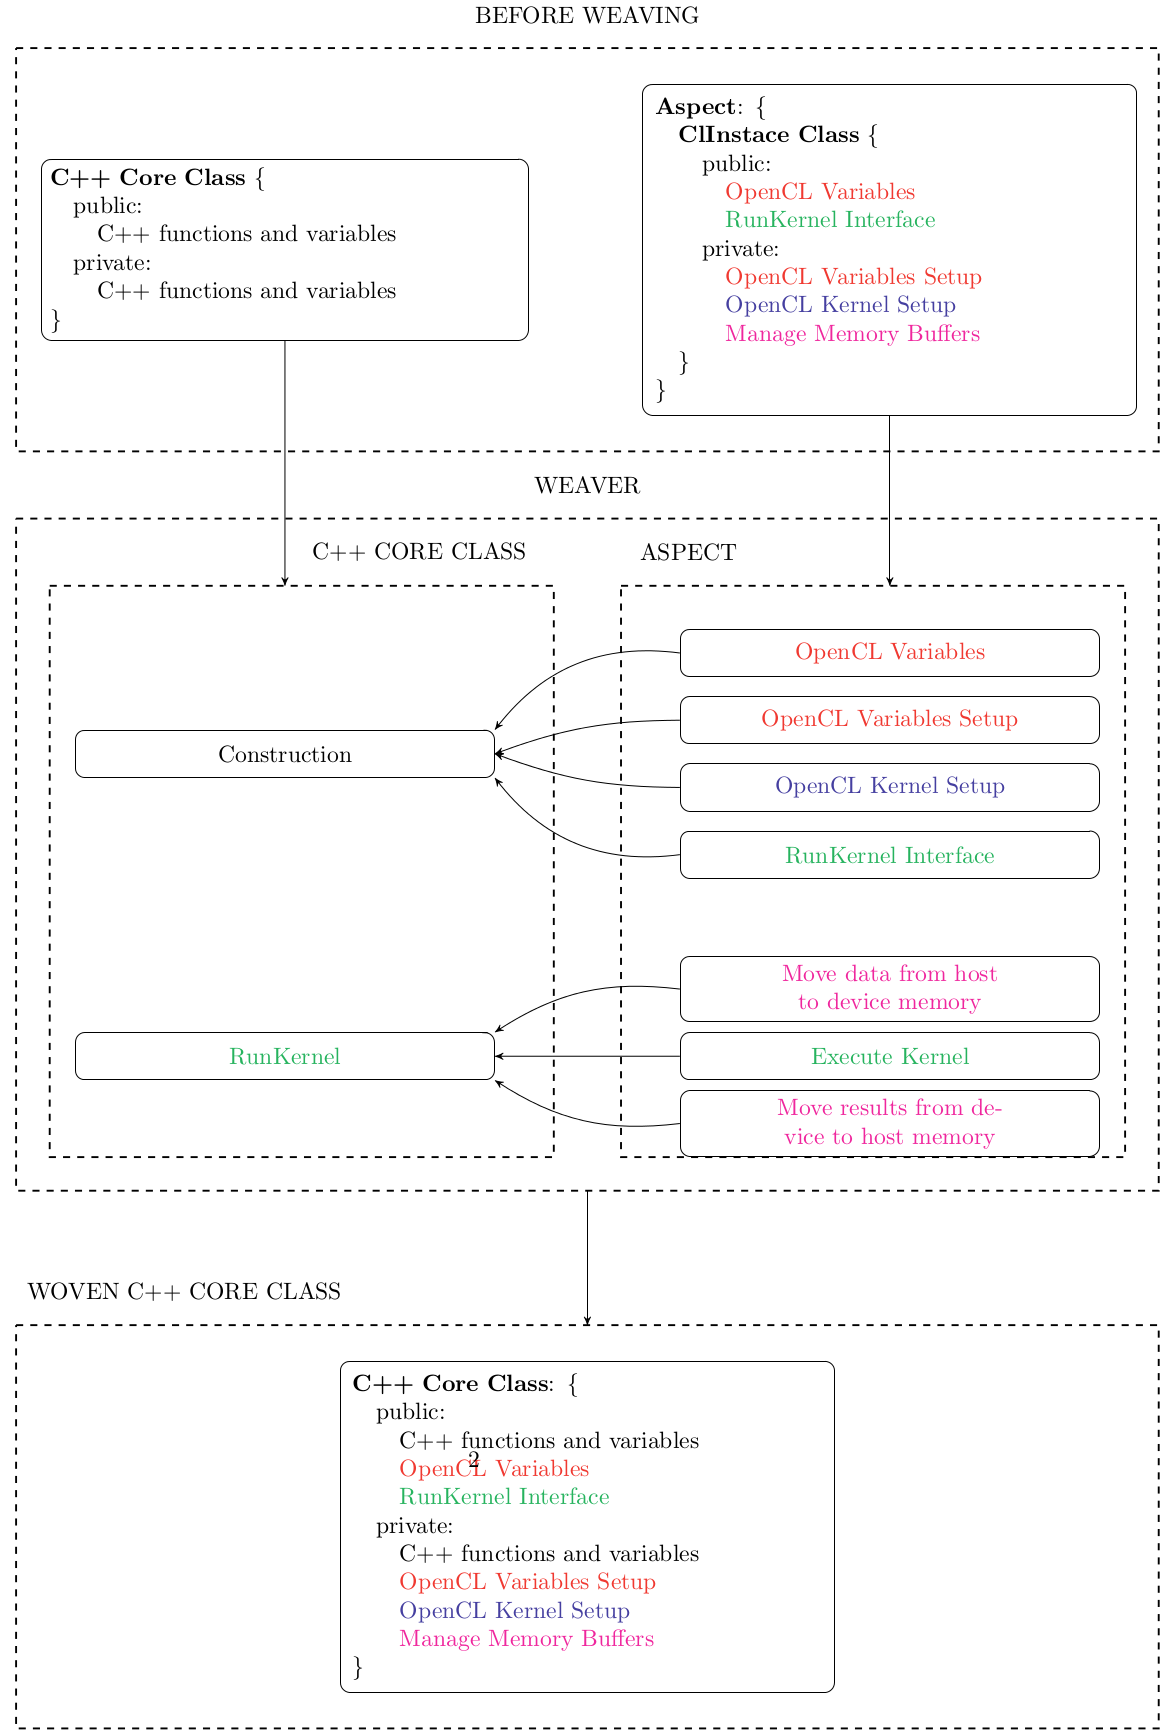
\includegraphics[width=0.49\textwidth]{weaving}
	\caption{High-level overview of the weaving process for the CAPP
		model. The output of the weaving process produces the code for
	compilation.}
	\label{fig:weaving}
\end{figure}

\subsection{Abstract ClContext Aspect}

Aspect\CPP is based on C++ and hence provides functionality for both inheritance
and polymorphism. The CAPP model makes use of these features and defines
an abstract aspect, the \textit{ClContext} aspect, which provides the core \CPP code with 
the cross-cutting OpenCL components necessary for executing a parallel kernel.
The OpenCL  components, both variables and member functions, are defined in the abstract 
aspect and are inherited by the derived aspect. Any additional OpenCL
functionality (which may improve specific parallel implementations) can then be 
defined in the derived aspect. Polymorphism is provided by Aspect\CPP 
through virtual pointcuts, which were used in the abstract
ClContext aspect to define an interface for the derived aspect
to specify which \CPP classes require parallel capability.
The \textit{CoreClasses} pointcut in Listing~\ref{slice} shows this.
This abstract aspect provides all the necessary OpenCL functionality for a 
parallel-capable class, without defining which \CPP class 
the aspect functionality should be woven into. Listing~\ref{dslice} shows an
example of a derived aspect for a \CPP vector addition class (VectAddCppClass), 
which uses the virtual pointcut CoreClasses to define the \CPP class
into which the functionality must be woven.

\subsection{OpenCL Class Introduction}

Observing Listing~\ref{vectcl}, there are numerous OpenCL specific variables
(variables defined below the red comments) which are required to setup the 
OpenCL environment. These are only the necessary variables -- there are many
more which provide additional features for parallel programming.
Many of these variables must be modified or recreated each
time a new kernel needs to be executed, requiring a significant amount of 
overhead when compared to the \CPP version of Listing~\ref{vectcpp}.

Aspect\CPP provides the \textit{slice} feature for defining C++ classes within
aspects. Furthermore, it allows for \textit{advice} to be defined for a 
virtual pointcut. This advice can be implemented to use \CPP inheritance which
will allow the aspect weaver to weave the slice class as a base class for 
any \CPP classes, or to derive from any C++ classes. Using these features, the CAPP model defines the 
\textit{ClInstance} slice class within the abstract ClContext aspect.  
The ClInstance class has the cross-cutting OpenCL variables as public
variables, and the cross-cutting OpenCL operations as private member functions.
The weaver then weaves the ClInstance class to be a base class of the \CPP
classes defined by the CoreClasses pointcut so that the OpenCL variables 
are part of those \CPP classes. This is known as \textit{introduction} in
aspect-orientated programming.
Listing~\ref{slice} shows the ClInstance slice class within the abstract aspect,
as well as the cross-cutting variables (below the red comments as per 
Listing~\ref{vectcl}) and member functions which provide the cross-cutting
OpenCL setup functionality.

\begin{lstlisting}[caption=Abstract ClContext aspect which defines the OpenCL variables
required for parallel programming.,label=slice,float=[!t]]
// ClContext.ah
aspect ClContext {
	class ClInstance {
	public:
		<@\color{Red!85}{// OpenCL variables}@>
		vector<cl::Platform> platforms;
		vector<cl::Device>   devices;
		vector<cl::Buffer>   buffers
		cl::clContext        context;
		cl::CommandQueue     queue;
		cl::Kernel           kernel;
		cl::Program          program;
		// Other variables and functions 
	private:
		<@\color{Red!85}{// Setup OpenCL variables}@>
		void SetupOpenCl(string devType, string kSource);
		<@\color{Blue!85}{// Setup OpenCL kernel}@>
		void SetupKernel(string kSource, string kName);
		<@\color{Magenta!85}{// Manage buffers on kernel execution}@>
		void ManageBuffers(vector<vector<float>>* inputs,
		                   vector<vector<float>>* outputs);
	};
	// Interface for defining C++ classes
	pointcut virtual CoreClasses() = 0;

	// Specify ClInstance as baseclass of classes
	// defined by CoreClasses()
	advice CoreClasses() : baseclass(ClInstance);

  // Other aspect components
};
\end{lstlisting}

\begin{lstlisting}[caption=Derived aspect defining a \CPP class into which the OpenCL 
	functionality should be woven.,label=dslice,float=[!t]]
#include "ClContext.ah"
aspect VectAdd : public ClContext {
	// Define C++ class to weave
	// OpenCL functionality into
	pointcut CoreClasses() = "VectAddCppClass";
};
\end{lstlisting}

\subsection{OpenCL Setup Function Introduction}

Again observing Listing~\ref{vectcl}, a large amount of the cross-cutting code
comes from the operations on the OpenCL variables. These operations (below the
red comments in the Listings) are for the setup of the OpenCL environment, and 
determine the available devices and platforms, and create the OpenCL context. They
cross-cut the \CPP code since they are not directly related to the intention of the
program and will need to be reimplemented for any class that is parallelised. Furthermore, 
these operations are generic - they are the same for any 
OpenCL program - allowing them to be defined as functions of the ClInstance
slice class. The operations for creating the kernel (below the blue 
comments in Listings) have the same problems and can therefore also be defined
as functions of the ClInstance slice class. 

The ClContext aspect then defines the \textit{ClSetup} pointcut to
specify where in the \CPP classes these functions should be executed. The
CAPP model defines the functions to be executed on construction of the
\CPP class. This is done so that once the C++ class has been instantiated,
all OpenCL variables will have been initialized to the appropriate values to allow
parallel computation from the \CPP class. 

To provide the programmer with flexibility regarding the parallel context,
the ClSetup advice makes use Aspect\CPP's \textit{tjp} pointer. 
The tjp pointer provides the aspect with access to the \CPP class, 
into which the aspect will be woven. Using \textit{tjp->that()} in an aspect 
is equivalent to using \textit{this} within a \CPP class . This feature was used 
to allow the programmer to specify the computation device (CPU or GPU), the 
kernel source file, and kernel name as arguments of the \CPP class constructor. 
Using tjp->that() allows the aspect to use the values provided by the 
programmer from the \CPP class. The aspect can then set up the OpenCL environment
to the programmer's preference.
Listing~\ref{clsetup} shows the definition of ClSetup pointcut, and its 
advice which calls the private member functions of the ClInstance
class, as defined in Listing~\ref{slice}.

\begin{lstlisting}[caption=Abstract aspect with the pointcut and advice for
OpenCL setup.,label=clsetup,float=[!t]]
// ClContext.ah
aspect ClContext {
	class ClInstance {
		// As per Listing 3 ...
	};
	// Other pointcuts and advice

	// Pointcut which defines where the OpenCL
	// setup function should be woven
	pointcut ClSetup = construction(CoreClasses());
  
	// Advice specifying how the OpenCL
	// setup functions should be woven
	advice ClSetup() : around() {
		<@\color{Red!85}{// Setup OpenCL variables}@>
		tjp->that()->SetupOpenCl(
			tjp->that()->devType, tjp->that()->kSource);
		<@\color{Blue!85}{// Setup OpenCL kernel}@>
		tjp->that()->SetupKernel(
			tjp->that()->kSource, tjp->that()->kName); 
		// Continue with core class constructor
		tjp->proceed();
	}
};
\end{lstlisting}

\subsection{RunKernel Interface}

Executing the kernel is the main component of a parallel application. Before the
kernel is run, the data on which the kernel operates must be moved from the
memory of the host to the memory of the device. Once the
kernel has finished executing, the results reside in the memory of the
device and are not available to the host until transferred
back from the device memory to the host memory. In OpenCL this
is done using the cl::Buffer type and specifying if the device memory
must be read from or written to. These operations are shown in Listing~\ref{vectcl} 
below the magenta comments. 

This process of memory allocation, movement, and
deallocation on each call of the kernel is not required for a \CPP implementation
and therefore cross-cut's the program's main intention. Furthermore, memory management 
is difficult in the C and \CPP languages because it is the programmer's
responsibility. This is magnified by the introduction of the device memory. 
As these operations are required each 
time the kernel is executed, the amount of cross-cutting code growing linearly 
with the number of kernels and kernel calls. 

These problems are solved by the CAPP model through aspects by defining
a pure virtual \textit{RunKernel} function in the ClInstance slice class. 
Since the ClInstance slice class will be a baseclass of any \CPP class requiring parallel 
functionality, the RunKernel function implementation must be defined in the 
\CPP class. By defining the RunKernel function as a pure virtual
function the aspect knows the structure of the function, which allows the 
ClContext aspect to define advice which can use the arguments passed to
the RunKernel function by the programmer, to perform the cross-cutting 
memory management code each time the RunKernel function is called from
the \CPP class.

The RunKernel function specifies that the arguments provided to it from the
\CPP code must be vectors of vectors, which hold data vectors for each input and
output of the kernel. This was influenced by the OpenCL API, which can only
operate on simple data structures (pointers, constants and OpenCL vector data
types), rather than complex data structures (C++ maps for example). 
By using vectors of vectors, the RunKernel interface can take any 
number of inputs and outputs, and each of these inputs and outputs can have any
number of elements, providing the programmer with a lot of flexibility from the
\CPP class. The more complex C++ vector data structure is then accessed through
pointers by the RunKernel advice to create OpenCL buffers, which the OpenCL kernel 
can operate on. This allows the \CPP class defined 
by the programmer to execute a kernel by simply calling the RunKernel function and 
passing the inputs and outputs as function arguments, as shown by Listing~\ref{crunkernel}. 
The tjp pointer is  used again by the aspect, but this time to access the RunKernel 
function arguments, and hence the input and output data for the kernel so that the memory can be
appropriately managed between the host and device.

Listing~\ref{runkernel} shows the \textit{ManageKernel} pointcut and advice,
which calls the \textit{ManageBuffers} function in the ClInstance
class, to perform the cross-cutting memory management between the host and
device before the RunKernel function is called from the \CPP
class.

\begin{lstlisting}[caption=Abstract aspect components which hide kernel
cross-cutting concerns.,label=runkernel,float=[!t]]
// ClContext.ah
aspect ClContext {
	class ClInstance {
	public:
		<@\color{Red!85}{// OpenCL variables ...}@>
		<@\color{Green!85}{// Execute kernel}@>
		virtual void RunKernel(
			vector<vector<float>>& inputs,
			vector<vector<float>>& outputs) = 0;
	private:
		<@\color{Red!85}{// Setup OpenCL variables ...}@>
		<@\color{Blue!85}{// Setup OpenCL kernel ...}@>
		<@\color{Magenta!85}{// Manage memory buffers}@>
		void ManageBuffers(
			vector<vector<float>>* inputs,
			vector<vector<float>>* outptus);
	};
	// Other advice and pointcuts 

	// Pointcut defines where the memory 
	// buffers should be managed
	pointcut ManageKernel() = 
		// Syntax means to weave ManageKernel advice 
		// into any RunKernel function in CoreClasses 
		execution("% ...::...::RunKernel(...)") &&
		within(CoreClasses());

	// Advice specifies how to manage buffers
	advice ManageKernel() : before() {
		<@\color{Magenta!85}{// Manage memory buffers}@>
		tjp->that()->ManageBuffers(tjp->arg<0>(),
								   tjp->arg<1>());
  }
};
\end{lstlisting}

\begin{lstlisting}[caption=Execution of a pallel kernel from a \CPP class.,label=crunkernel,float=[!t]]
void VectAddCpp(int argc, char** argv) {
	<@\color{Green!85}{// Instantiate vect addition class }@>
	ParVectAddCppCore vectAdd;
	<@\color{Green!85}{// Create input and output buffers}@>
	vector<vector<float>> inputs;
	vector<vector<float>> outputs;
	<@\color{Green!85}{// Fill vectors with data ...}@>
  
	<@\color{Green!85}{// Execute kernel}@>
	vectAdd.RunKernel(inputs, outputs);
}
\end{lstlisting}

\section{Results}\label{sec:results}

This section presents the results of application of the CAPP model to two
GPGPU programming problems. The first problem is known as SAXPY
(Single-precision a*X + Y) \cite{harris:saxpy}, and is relatively 
simple to implement in parallel. The second problem is the evaluation of option 
prices using the Black-Scholes option pricing model \cite{gems:blackscholes},
which is more complex than the SAXPY problem, and hence applies the CAPP model 
to more `tangled' \CPP code. Results are given for both the performance and
number of lines of code for the CAPP, \CPP (CPU only), and OpenCL
implementations to demonstrate both the performance capabilities and the code
simplification a CAPP implementation can provide. For each implementation 50
runs were performed. The results shown are an average of the 50 runs. An Intel 
i7-3635QM (2.4GHz, quad-core, 6M cache) CPU was used for the CPU
implementations and an Nvidia GeForce GT 650M (384 cores, 900Mhz) GPU was used for
the CAPP and OpenCL implementations.

\subsection{SAXPY Problem}


\begin{figure}[!t]
	\centering
	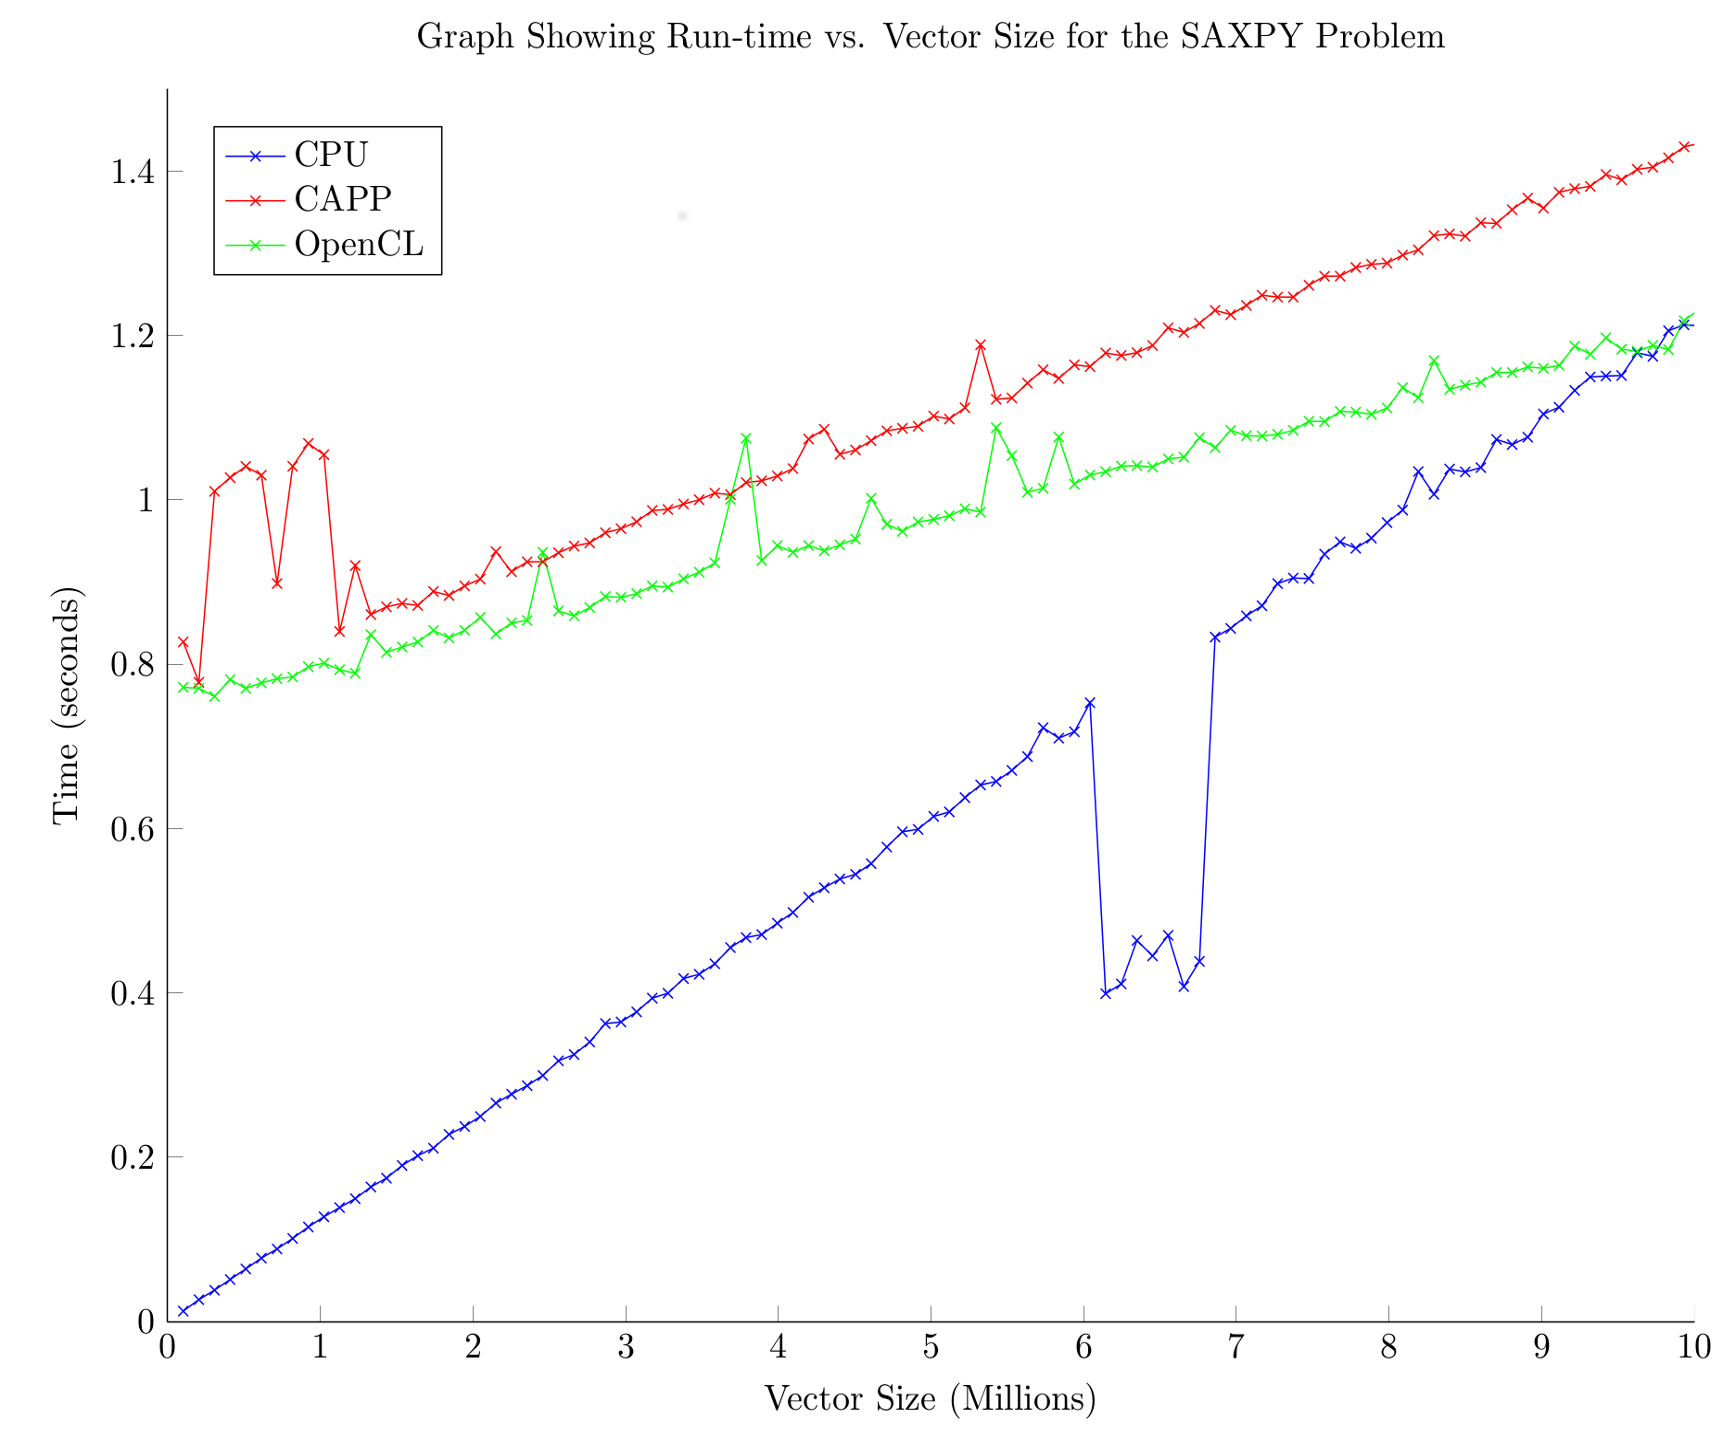
\includegraphics[width=0.46\textwidth]{Saxpy}
	\caption{Results for the three implementations of the SAXPY problem. Lower
	values are better.}
	\label{fig:saxpy}
\end{figure}

\begin{table}[!b]
\centering
\caption{Comparison of the number of lines of code per file type for the SAXPY
problem.}
\label{tab:saxpy}
\begin{tabular}{|c|c|c|c|} 
	\hline
				& CAPP			& OpenCL		& \CPP	\\ \hline
.h				& 48			& 0				& 38	\\ \hline
.cpp			& 43			& 152			& 73	\\ \hline
.cl				& 5				& 5				& 0		\\ \hline
.ah				& 53			& 0				& 0		\\ \hline
.cc				& 78			& 0				& 0		\\ \hline
\textbf{Total}	& \textbf{227}	& \textbf{157}	& \textbf{111}		\\ \hline		
\hline
\end{tabular}
\end{table}

Various vector sizes were used and the run-time of each of the implementations
was measured to validate that the solution using the
CAPP model scales similarly to the OpenCL implementation. Figure~\ref{fig:saxpy} 
shows the results for the run-time of each implementation. Transferring
the data between the CPU and the GPU is a large initial overhead for the SAXPY problem
\cite{gregg:saxpy}. This is evident by the offset of the
OpenCL and CAPP results for small vector sizes. Since the CPU implementation
doesn't require data transfer to an external device the offset is not present.
The gradient of each of the results provides important information as it shows
how each of the implementations scale with an increase in the data size. 
The gradient of the CAPP (0.61) and OpenCL (0.48) solutions are comparable, with
the CAPP solution being slightly worse. The gradient of the \CPP
implementation (1.19) is considerably worse and does not scale particularly
well. The average performance of the CAPP implementation was 7\% slower
than the OpenCL implementation with the worst case performance being 21\%
slower.

The second performance metric is the number of lines
of code of each implementation. The results are shown in 
Table~\ref{tab:saxpy}. The important files are the \CPP (.h, .cpp) and kernel (.cl)
files as these are what the programmer will need to write. The aspect files (.ah, .cc) are
part of the CAPP model and do not need to be re-implemented by the programmer. 

\subsection{Black-Scholes Option Pricing Problem}

This problem requires evaluating option prices using the Black-Scholes 
model for options pricing and is a good example of an application of the CAPP 
model to a real world problem. The number of options was varied and the
run-time was measured for the each implementation, the results are shown in 
Figure~\ref{fig:blackscholes}. 
This example illustrates level of performance the CAPP model can
provide. The CAPP and OpenCL run-times are very similar. The average 
performance of the CAPP implementation was 1.4\% slower than the
OpenCL implementation, while the \CPP implementation was up to 9 times slower
than both the CAPP and OpenCL implementations.

\begin{figure}[!t]
	\centering
	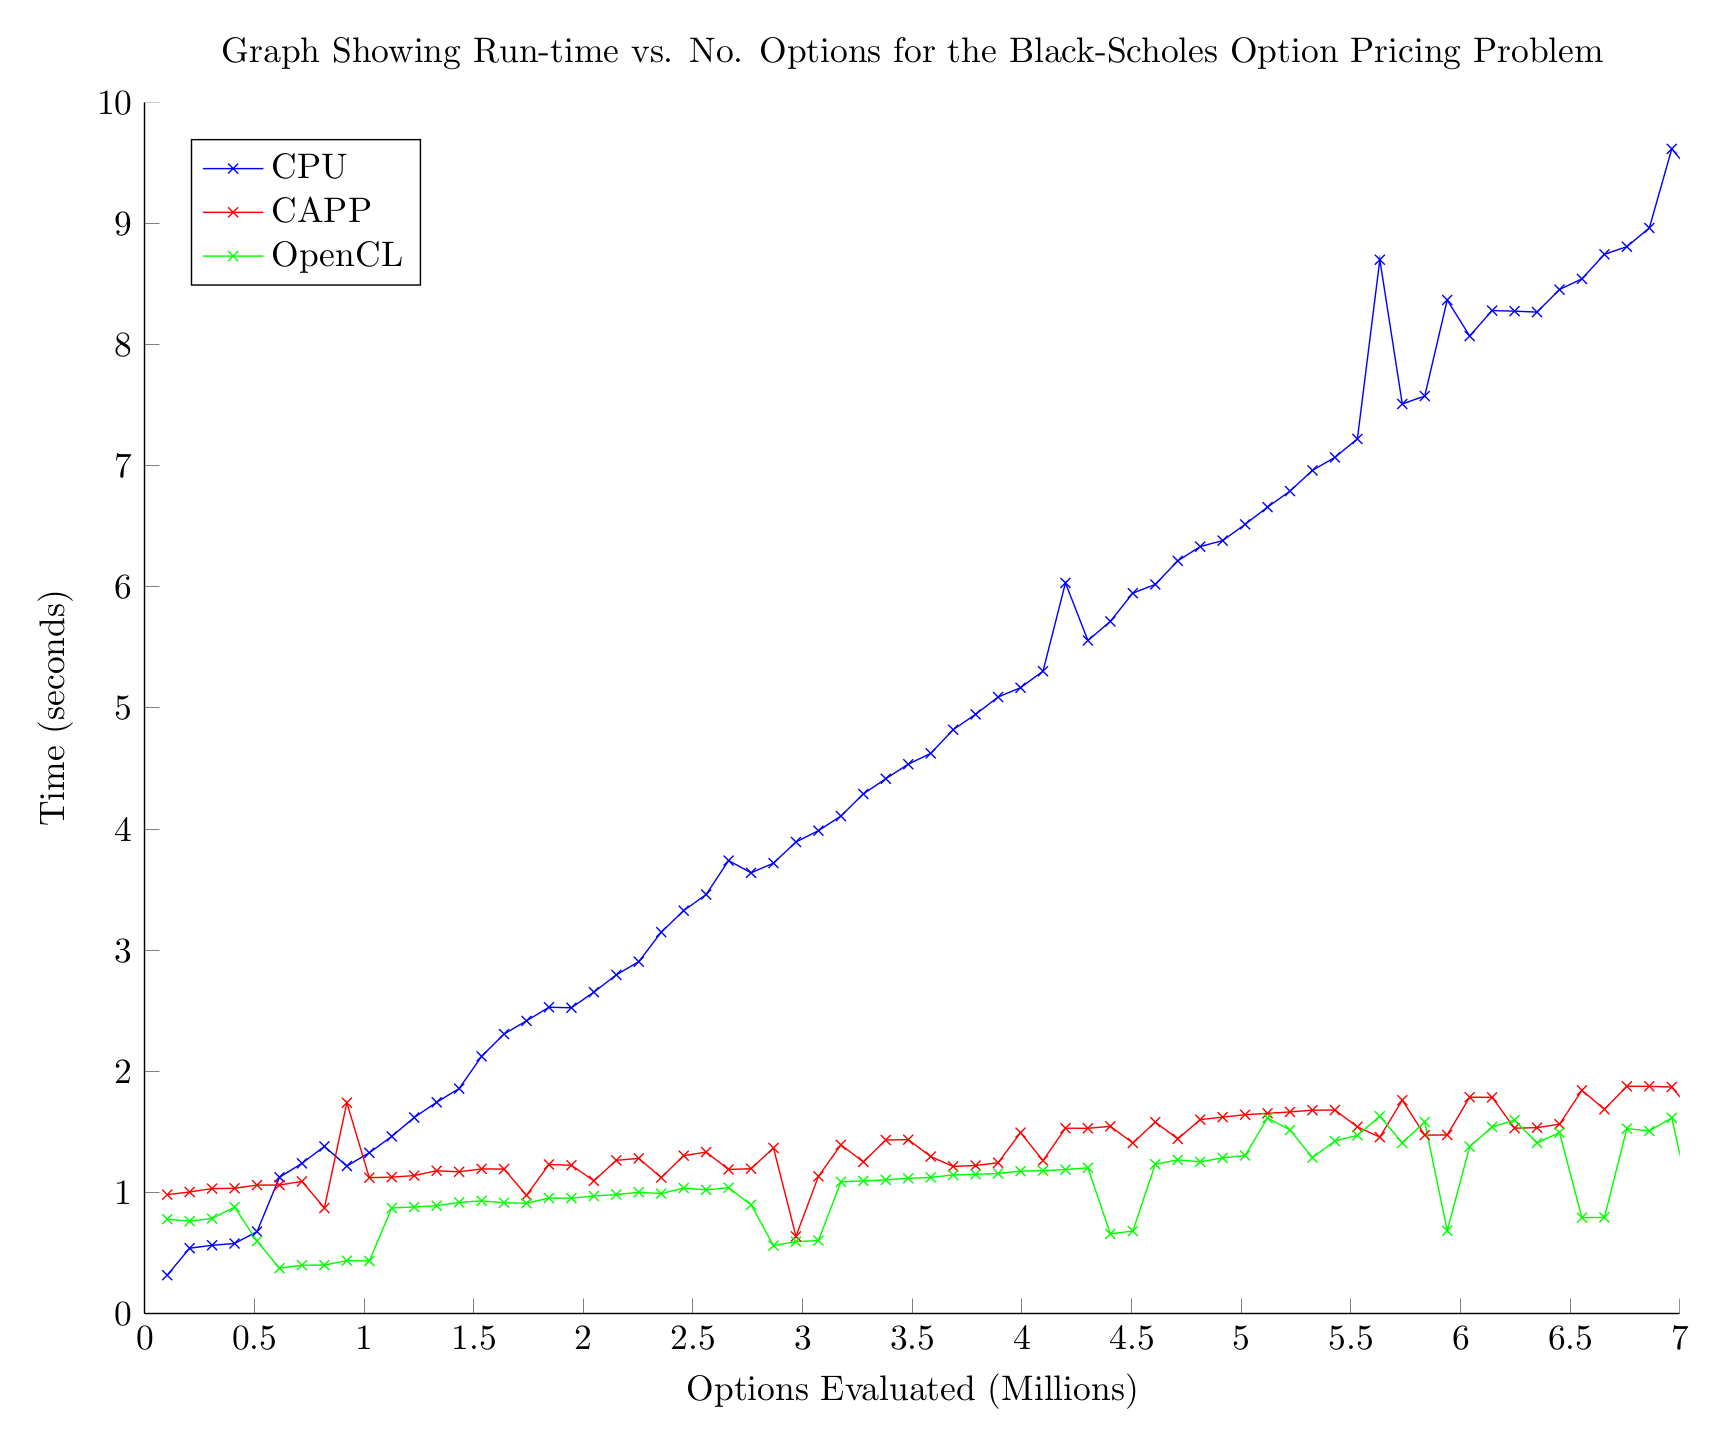
\includegraphics[width=0.45\textwidth]{BlackScholes}
	\caption{Results for the three implementations of the Black-Scholes option
		evaluation problem. Lower values are better.}
	\label{fig:blackscholes}
\end{figure}

The comparison of the number of lines of code for each of the implementations is
shown in Table~\ref{tab:blackscholes}. The file types of interest are the same as 
those mentioned in the SAXPY example. 

\begin{table}[!b]
\centering
\caption{Comparison of the number of lines of code per file type for the
Black-Scholes option pricing problem.}
\label{tab:blackscholes}
\begin{tabular}{|c|c|c|c|} 
	\hline
				& CAPP			& OpenCL		& \CPP		\\ \hline
.h				& 37			& 0				& 32		\\ \hline
.cpp			& 55			& 181			& 121		\\ \hline
.cl				& 73			& 73			& 0			\\ \hline
.ah				& 53			& 0				& 0			\\ \hline
.cc				& 78			& 0				& 0			\\ \hline
\textbf{Total}	& \textbf{296}	& \textbf{254}	& \textbf{153}		\\ \hline		
\hline
\end{tabular}
\end{table}


\section{Evaluation and Limitations}\label{sec:evaluation}

\subsection{Analysis of Results}

The results show some dips and spikes for both the SAXPY and Black-Scholes
problems. These can be caused by both temperature changes and the effectiveness
of compiler optimisations for the data size. The 50 runs of each implementation
were performed to reduce these effects as much as possible.

The results presented in the Section~\ref{sec:results} show the similarity in
the performance of a CAPP implementation and an OpenCL implementation, as
well as the performance advantage over a \CPP, CPU only implementation. The
similarity of the CAPP and OpenCL performance proves the viability of
using the CAPP model for parallel programming. The number of lines of 
code comparison provides further justification for using a CAPP
implementation as the number of lines of \CPP code were dramatically
reduced, requiring only 91 lines and 92 lines of \CPP code for the SAXPY and
Black-Scholes CAPP implementations respectively.
Furthermore, the resultant \CPP code is modular and hence easily maintainable, 
which is typically not the case for OpenCL code. Therefore,
the CAPP implementation code was more comparable to the \CPP code,
both structurally and in length. The CAPP model thus provides
performance comparable to an OpenCL implementation but written in modular \CPP.

\subsection{Advantages}

The CAPP model provides numerous advantages which should be mentioned.

Low-level parallel programming complexities are hidden from the programmer using aspects. 
This results in \CPP code which has no components that cross-cut the code's intention, as 
well as kernel functions which can be executed from the \CPP code with a single
function call through the RunKernel interface. 

The RunKernel interface provides flexibility to the programmer through the use
of vectors. Any number of inputs and outputs arguments can be specified due to
the dynamic nature of vectors. Each of these inputs and outputs can have any 
dimension, and the dimensionality of the inputs and outputs can vary.

While the OpenCL functionality is hidden from the programmer by the aspects,
this code is still available to the programmer if desired. This is could be
beneficial in many scenarios, for example where a team is using the
CAPP model GPU experts could modify the implementation provided by the
CAPP model to improve performance but non-GPU experts could still use
the \CPP interface.  

There is negligible loss in performance since the aspects are woven into the
\CPP code before compilation and hence do not have run time implications other
than the necessary OpenCL related work.

The use of Aspect\CPP results in the CAPP model being capable of
providing general Aspect-Oriented Programming support for \CPP. The benefit of this is that
large-scale applications could use standard Aspect\CPP to modularize other
cross-cutting concerns from the \CPP application, logging for example, and using the
CAPP model to improve the performance of critical areas of the
application, in \CPP.

The CAPP code which performs all the OpenCL components is reliable.
A developer would not have to debug the OpenCl setup and memory management code
when testing a parallel algorithm. Furthermore, the \CPP code is simple. These
features results in a faster overall parallel programming development cycle and
limits potential sources of error to the kernel function provided by the
programmer.

\subsection{Limitations}

Due to the weaving process occurring before compilation, it was expected that
the CAPP implementation would provide performance equal to that of the
OpenCL implementation. However, the results showed a marginal performance
reduction. This was determined to be due to Aspect\CPP weaver producing code
which compiles to a slightly less efficient executable. 

Since Aspect\CPP is still in the development process it does not support all 
the features of \CPP, for example generic programming through templates, within
aspects. 
This places a limitation on the \CPP code  the programmer may write if they 
are using the CAPP model. The development of the Aspect\CPP compiler 
is therefore a limitation of the CAPP model as the latest \CPP 
features will not be available. However, future releases of the Aspect\CPP
compiler are scheduled to include support for many more modern \CPP features.

\section{Conclusion}\label{sec:conclusion}

This paper described the CAPP model which uses aspects to remove
cross-cutting code from the \CPP code, thereby providing simpler, more modular
parallel capable \CPP code. The aspects were implemented using AspectC++,
and the parallel functionality was implemented using OpenCL. The cross-cutting 
components handled by the aspect are the setup of the OpenCL
context, the compilation of the kernel, the transfer of memory between the 
host and device when the kernel is executed, and the kernel execution itself. 
The aspect defined by the CAPP model is abstract and can be used for 
any parallel programming application. An interface is provided for calling the 
OpenCL kernel from the \CPP code so that no cross-cutting OpenCL code is present in
the \CPP code, and the developer is not required to learn the OpenCL API. The
kernel is left to be written by the developer since it is specific to the
application. This is similar to most existing solutions, however, the existing
solutions require operations to be defined using the proposed language or
framework, which operate on data in a parallel manner, rather than requiring an
OpenCL or CUDA kernel.

Two example problems were looked at: SAXPY and options pricing. CAPP, OpenCL 
and \CPP implementations were compared for each problem. The performance of the 
CAPP model was shown to be similar to that of the OpenCL
implementation, with 7 and 1.4\% performance reductions, respectively. Structurally 
the CAPP implementation was similar 
to the \CPP  implementation in terms of the number of lines and modularity, and
better designed than the OpenCL implementation. Both CAPP implementations
required no OpenCL code in the \CPP header or implementation files, therefore the
CAPP model provides high performance parallel programming using \CPP.

\section{Future Work}\label{sec:future}

The CAPP model proposed in this paper looked at using aspects to hide
the complexities and cross-cutting concerns of parallel programming. However, only a
minimal amount of the OpenCL API was used to allow OpenCL kernels to be run from the
\CPP code. The OpenCL API is extensive and provides many additional features which 
could are ideal candidates for encapsulation with aspects, such as timing,
tracing, and performance profiling, to name a few. More specific aspects could
provide these features as well as deriving from the abstract aspect, providing
the additional features of the OpenCL API.

The slight performance reduction of the CAPP implementation over the
OpenCL implementation could be reduced by optimising the aspect code.

OpenCL provides functionality which is available for parallel devices from
multiple vendors, which may not take advantage of features specific to some
vendors - for example dynamic parallelism available to some Nvidia GPUs.
Future work would involve extending the CAPP aspects to take advantage
of these specific hardware features. This would require including the CUDA API
into the model. To perform this efficiently templates would need to be used, and
hence the next release of the Aspect\CPP compiler would be required, to
minimise run time evaluation and rather perform the evaluation at compile time.

To provide a parallel programming environment which can be written explicitly in
\CPP, the kernel would need to be written using C++. Future versions of the
CAPP model could provide the option to the programmer to either specify
the kernel themselves, or to have the CAPP model attempt to
parallelize a \CPP function into a kernel. It is unlikely that this feature would
ever achieve performance levels equivalent to kernels specified by experienced
programmers. However, even if only minimal speedup were to be achieved, this would prove 
useful for applications where any additional performance is needed but where the
programmers have no knowledge of parallel programming. 

%
% The following two commands are all you need in the
% initial runs of your .tex file to
% produce the bibliography for the citations in your paper.
\bibliographystyle{abbrv}
\bibliography{sigproc}  % sigproc.bib is the name of the Bibliography in this case
% You must have a proper ".bib" file
%  and remember to run:
% latex bibtex latex latex
% to resolve all references
%
% ACM needs 'a single self-contained file'!
%
%CAPPENDICES are optional
%\balancecolumns
%Appendix A
%\balancecolumns % GM June 2007
% That's all folks!
\end{document}
